\documentclass[serif, aspectratio=169]{beamer}
%\documentclass[serif]{beamer}  % for 4:3 ratio

\RequirePackage{minted2}
\usepackage[T1]{fontenc} 
\usepackage[utf8]{inputenc}
\usepackage{fourier} % see "http://faq.ktug.org/wiki/uploads/MathFonts.pdf" for other options
\usepackage{hyperref}
\usepackage{latexsym,amsmath,xcolor,multicol,booktabs,calligra}
\usepackage{graphicx,pstricks,listings,stackengine}
\usepackage{lipsum}
\usepackage{../HKUSTstyle}

%imports customs%
\usepackage{caption}    % for subfigures
\usepackage{subcaption} % for subfigures
\usepackage{ragged2e}
\usepackage{booktabs,makecell}
\usepackage{colortbl}
\usepackage{multirow}
\usepackage{cite}
\usepackage{tcolorbox}
\usepackage[sort,authoryear]{natbib}

\author{Julien Bezançon}

\title{Python Programmation}
\subtitle{CM 7~: Second Course Recap}

\institute{julien.bezancon@univ-lorraine.fr / \url{https://julienbez.github.io}}

\date{}

% defs
\def\cmd#1{\texttt{\color{red}\footnotesize $\backslash$#1}}
\def\env#1{\texttt{\color{blue}\footnotesize #1}}

% set colors
\definecolor{hkustyellow}{RGB}{167, 131, 55}
\definecolor{hkustblue}{RGB}{0, 56, 116}
\definecolor{hkustred}{RGB}{209, 51, 59}

\lstset{
    basicstyle=\ttfamily\small,
    keywordstyle=\bfseries\color{deepblue},
    emphstyle=\ttfamily\color{deepred},    % Custom highlighting style
    stringstyle=\color{deepgreen},
    numbers=left,
    numberstyle=\small\color{halfgray},
    rulesepcolor=\color{red!20!green!20!blue!20},
    frame=shadowbox,
}

\begin{document} %  --- --- --- --- --- --- --- --- --- --- --- --- 

\begin{frame}[noframenumbering,plain]
    \titlepage
    \vspace*{-0.6cm}
    \begin{figure}[htpb]
        \begin{center}
            \hspace{0.3cm}
            
\includegraphics[width=0.7\columnwidth]{../../../IMAGES/loria_idmc.png}
        \end{center}
    \end{figure}
\end{frame}

% \begin{frame}    
%     \tableofcontents[sectionstyle=show,
%     subsectionstyle=show/shaded/hide,
%     subsubsectionstyle=show/shaded/hide]
% \end{frame}

\begin{exoframe}
    \begin{center}
        \Large
        During this recap, we will correct exercises \\
        from previous practical sessions. \\
        \vspace{15pt}
        Short exercises: using the board. \\
        Long exercises: by group (10 groups max).
    \end{center}
\end{exoframe}

\begin{frame}{CM5 Doggy bag}
    \begin{minipage}{0.45\columnwidth}
        \begin{block}{File handling}
            \begin{itemize}
                \item Open and write a file
                \item Encoding and pathing
                \item String parsing
                \item Dedicated libraries
            \end{itemize}
        \end{block}
        \begin{block}{File navigation}
            \begin{itemize}
                \item File VS python structures
                \item Common errors
            \end{itemize}
        \end{block}
    \end{minipage}
    \hfill
    \begin{minipage}{0.45\columnwidth}
        \begin{figure}
            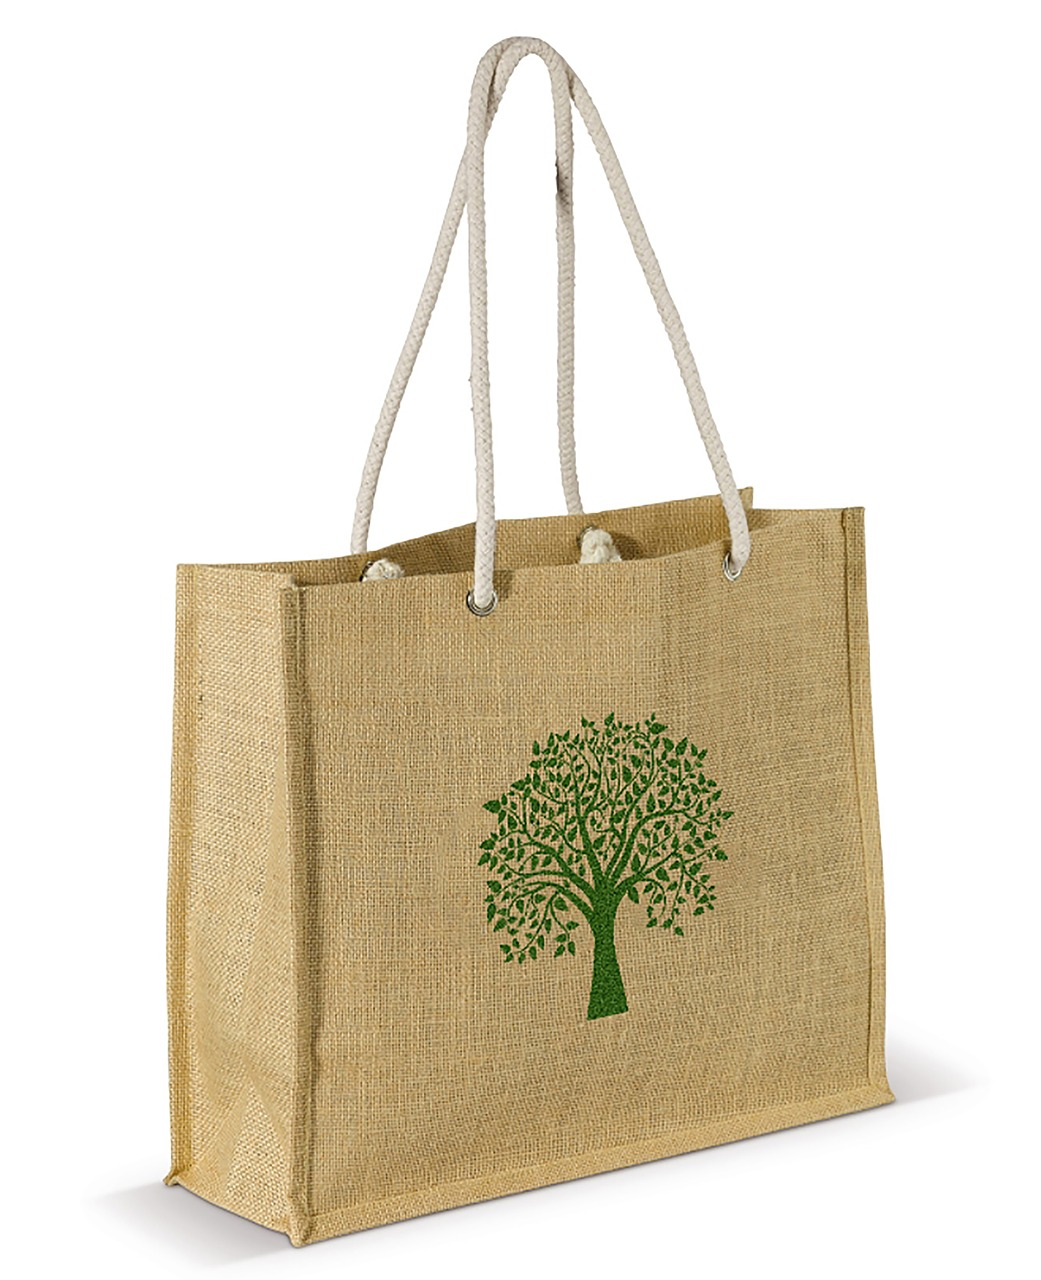
\includegraphics[width=0.9\columnwidth]{../../../FIGURES/divers/doggybag.jpg}
        \end{figure}
    \end{minipage}
\end{frame}

\begin{frame}{CM6 Doggy bag}
    \begin{minipage}{0.45\columnwidth}
        \begin{block}{Libraries}
            \begin{itemize}
                \item The toolboxes of python
                \item pandas, sklearn and matplotlib
            \end{itemize}
        \end{block}
        \begin{block}{Virtual env}
            \begin{itemize}
                \item Use them !
                \item Global venv = BAD
            \end{itemize}
        \end{block}
        \begin{block}{Modules}
            \begin{itemize}
                \item Snippets of code
                \item Better code structure
            \end{itemize}
        \end{block}
    \end{minipage}
    \hfill
    \begin{minipage}{0.45\columnwidth}
        \begin{figure}
            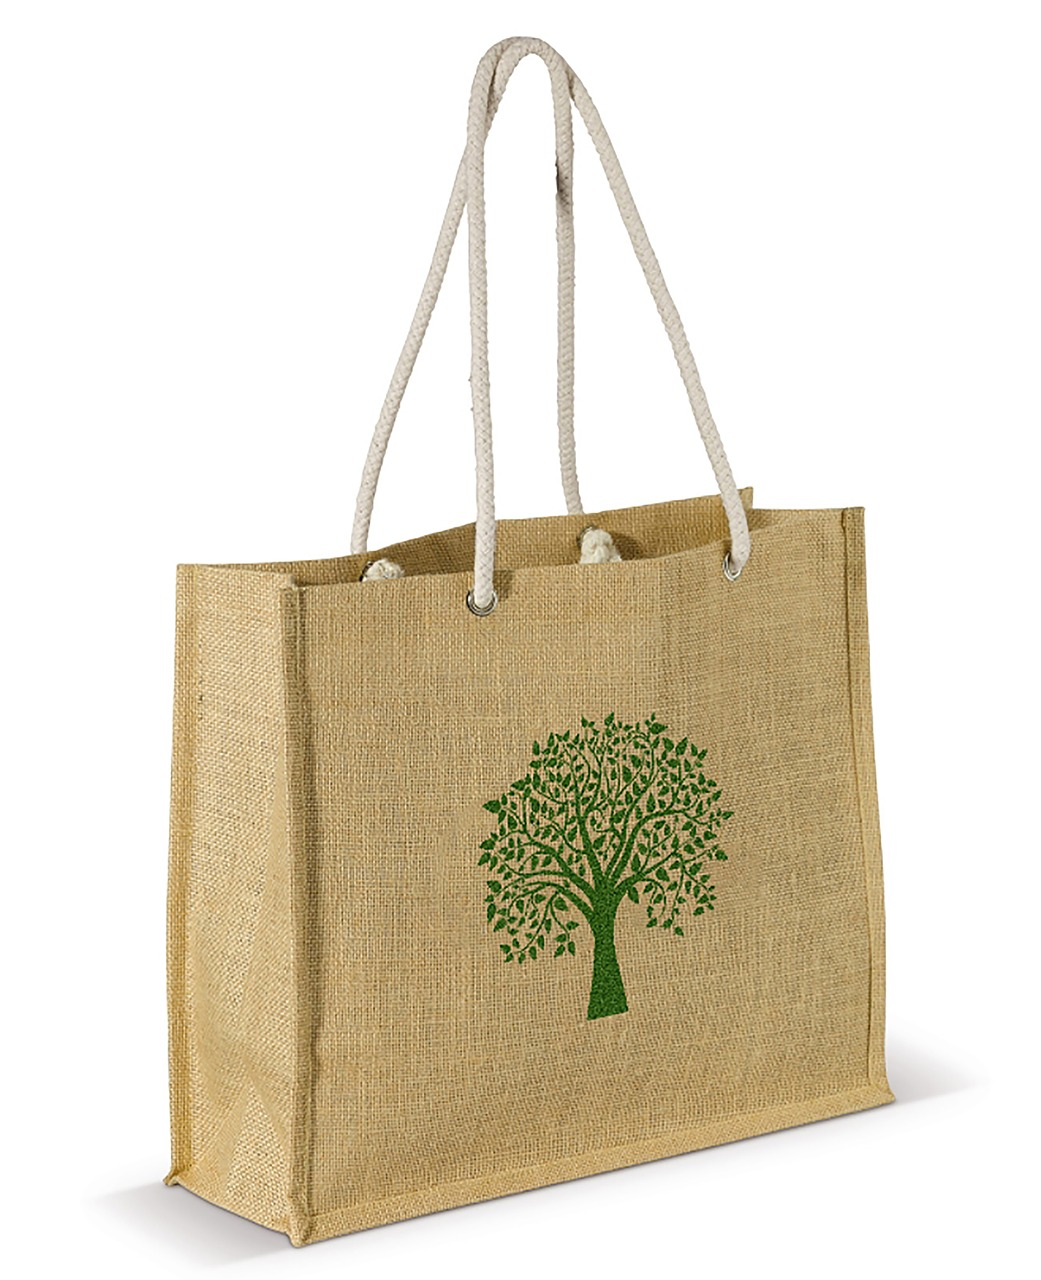
\includegraphics[width=0.9\columnwidth]{../../../FIGURES/divers/doggybag.jpg}
        \end{figure}
    \end{minipage}
\end{frame}

\begin{exoframe}
    \begin{center}
        \Large
        Let's proceed to the corrections !
    \end{center}
\end{exoframe}

\begin{exoframe}
    \begin{center}
        \Large
        Now, let's play a game... \\
        Can you guess the result of the following scripts ? \\
    \end{center}
\end{exoframe}

\begin{frame}[fragile]{First Guess}
    \begin{pythoncode}
    data = [
        "file1",
        "file2"
        "file3"
    ]

    print (len (data))
    \end{pythoncode}
    \vfill
    \pause
    \begin{itemize}
        \item No error, but this list only has two elements
        \item Do not forget the commas !
    \end{itemize}
\end{frame}

\begin{frame}[fragile]{Second Guess}
    \begin{pythoncode}
    def f (x):
        return (x+y)

    y = 2
    print (f(3))
    \end{pythoncode}
    \vfill
    \pause
    \begin{itemize}
        \item No error, return 5
        \item Refer to python scopes if needed
    \end{itemize}
\end{frame}

\begin{frame}[fragile]{Third Guess}
    \begin{pythoncode}
    if 2 < 4 > 3 < 5:
        print("simple")
    
    if 2 < 4 > 3 < 5:
        print("simple")
    \end{pythoncode}
    \vfill
    \pause
    \begin{itemize}
        \item Will return "simple" and nothing, respectfully
        \item To read from left to right
    \end{itemize}
\end{frame}

\begin{frame}[fragile]{Fourth Guess}
    \begin{pythoncode}
    a = [print(i) for i in range(10)]
    print(a)
    \end{pythoncode}
    \vfill
    \pause
    \begin{itemize}
        \item Will print(i) each time, then a list of None
        \item use \wordbox{"".join()} to print a list instead
    \end{itemize}
\end{frame}

\begin{frame}[fragile]{Fifth Guess}
    \begin{pythoncode}
    a = 100
    b = 10**2
    print(a is b)

    a = 1000
    b = 10**3
    print(a is b)
    \end{pythoncode}
    \vfill
    \pause
    \begin{itemize}
        \item Print True, then False
        \item Why ? Take your guesses
    \end{itemize}
\end{frame}

\begin{frame}[fragile]{Sixth Guess}
    \begin{pythoncode}
    a = 0
    b = 0

    while a < 1000:
        check = a is b
        print(check)
        a += 1
        b += 1
    \end{pythoncode}
    \vfill
    \pause
    \begin{itemize}
        \item Print True up to 256
        \item Numbers from -5 to 256 have dedicated memory space
    \end{itemize}
\end{frame}

\begin{frame}[fragile]{Seventh Guess}
    \begin{pythoncode}
    x = 'abc'
    y = 'abc'
    print(x is y)

    x = 'abc!'
    y = 'abc!'
    print(x is y)
    \end{pythoncode}
    \vfill
    \pause
    \begin{itemize}
        \item Print True, then False
        \item Some strings have dedicated memory space
    \end{itemize}
\end{frame}

\begin{frame}[fragile]{Eight Guess}
    \begin{pythoncode}
    with open("toto.txt",'r') as f:
        for x in f:
            print(x)
    \end{pythoncode}
    \vfill
    \pause
    \begin{itemize}
        \item Print each line of "toto.txt"
        \item The iretator of an object is not always clear
    \end{itemize}
\end{frame}

\end{document}
